\documentclass{article}

% Use the NeurIPS 2025 style (preprint => non-anonymous, line-numbered draft).
% Switch to \usepackage{neurips_2025} for the anonymized submission build.
\PassOptionsToPackage{numbers, compress}{natbib}
\usepackage[preprint]{neurips_2025}

\usepackage[utf8]{inputenc}
\usepackage[T1]{fontenc}
\usepackage{hyperref}
\usepackage{url}
\usepackage{booktabs}
\usepackage{amsfonts}
\usepackage{amsmath}
\usepackage{amssymb}
\usepackage{nicefrac}
\usepackage{microtype}
\usepackage{xcolor}
\usepackage{graphicx}

% handy macros for the placeholders we will fill later
\newcommand{\TODO}[1]{\textcolor{red}{[\textbf{TODO:} #1]}}
\newcommand{\PH}[1]{\textcolor{blue}{[\,#1\,]}}
\newcommand{\sg}{\operatorname{sg}}
\newcommand{\real}{\mathrm{real}}

\title{W2F: One-Step Word to Face Generative Typography via Drifting}

\author{%
  Yuxuan Chen\thanks{Team leader} \\
  \And
  Junhao Huang \\
  \And
  Yanmohan Wang \\
}

\begin{document}
\maketitle

\begin{abstract}
We present \textbf{Words to Faces (W2F)}, a one-step generative framework that composes a
recognizable human face out of a fixed set of $K{=}12$ alphabet glyphs. A single feed-forward
generator predicts, for every glyph, both \emph{what} to draw (a small $32{\times}32$ letter image) and
\emph{where} to put it (an affine pose), and a Spatial Transformer Network (STN) places the glyphs onto
a $128{\times}128$ canvas. The model uses neither a GAN discriminator nor an iterative diffusion
sampler: it is trained \emph{only} by the recently proposed \textbf{Drifting} loss
\citep{lambert2026drifting}, a particle-based distribution-matching objective applied at two levels ---
a per-glyph signal that keeps each placed image on its letter manifold, and a composite signal that
pulls the whole canvas toward the distribution of real face line-drawings. We work in a deliberately
hard corner of the design space: one-step generation, no face-specific priors, and no paired
(text\,$\to$\,face) supervision. We give a complete, reproducible description of the architecture, the
two-level Drifting losses (with full pseudocode and every modification that distinguishes our variant
from the original objective), and the exact mathematical form of all eleven loss terms, the two data
pipelines, and the frozen models used for evaluation. Our central empirical finding is a sharp
\emph{legibility--realism trade-off}, which we characterize quantitatively, and we ablate our main
design choice, feature-wise letter conditioning (FiLM).
\end{abstract}

\section{Introduction}
\label{sec:intro}
Typography art --- arranging letters so that, viewed as a whole, they form a larger image such as a
face --- is a classic example of \emph{emergent} visual structure. Reproducing it automatically is
hard for two reasons. First, the elements are \emph{constrained}: each must remain a recognizable
letter, so the model cannot draw arbitrary strokes. Second, the global target (a face) and the local
target (a letter) live in different distributions that must be satisfied \emph{simultaneously} by the
same pixels.

Most modern generative models reach such targets through machinery we explicitly want to avoid. GANs
\citep{goodfellow2014gan} introduce a discriminator that is unstable to train and prone to mode
collapse; diffusion models \citep{ho2020ddpm} require many sequential denoising steps (which one-step
distillations such as consistency models \citep{song2023consistency} only partly remove). We instead
build on \textbf{Drifting} \citep{lambert2026drifting}, which trains a \emph{one-step} generator by
moving generated samples along score-like vector fields: toward the real-data manifold (an attraction
field $V_p$) and away from other generated samples (a repulsion field $V_q$). Drifting needs no
discriminator and no iterative sampler.

Within this paradigm we solve the typography-face problem under three constraints that define our
\textbf{design space}: (i) \textbf{one-step} generation (a single forward pass, no iterative
refinement); (ii) \textbf{no priors} --- no facial landmark templates, no hand-placed eye/nose/mouth
anchors, and no face-engineered similarity measures (generic structural measures such as
intersection-over-union, which know nothing about faces, are permitted); (iii) \textbf{no paired
data} --- the model never sees a (text\,$\to$\,face) pair; it is given one unpaired collection of real
face line-drawings and one unpaired collection of letters, and the Drifting objective is what bridges
them.

\paragraph{Contributions.}
(i) A one-step generator whose two-stage transformer is built to \emph{co-adapt with the STN}: the
predicted layout is fed both into the spatial transformer and back into the rendering stage
(Sec.~\ref{sec:arch}). (ii) A full, reproducible instantiation of Drifting at two hierarchical levels
with several modifications beyond the original algorithm, given as pseudocode and exact equations
(Sec.~\ref{sec:overview}--\ref{sec:loss}). (iii) A pure-drifting face-generation \emph{baseline} that
establishes the face-quality ceiling, documented end-to-end including the frozen models used for
evaluation (Sec.~\ref{sec:baseline}--\ref{sec:auxmodels}). (iv) A quantitative characterization of the
\emph{legibility--realism trade-off} and an ablation of feature-wise letter conditioning
(Sec.~\ref{sec:results}--\ref{sec:ablation}).

\section{Related work}
\label{sec:related}
\paragraph{One-step / distribution-matching generation.} Beyond GANs and diffusion, generators can be
trained by directly matching distributions, e.g.\ Maximum Mean Discrepancy \citep{li2015mmd},
optimal-transport divergences, and recently score- and particle-based ``drift'' objectives that push
one-step samples toward the data score \citep{song2019ncsn} without a learned critic
\citep{lambert2026drifting}. Our work
applies and stress-tests Drifting in a structurally constrained, compositional setting.
\paragraph{Typography and artistic text rendering.} Generating images out of glyphs spans
structure-based ASCII art \citep{xu2010ascii}, calligram layout, and neural semantic typography that
deforms letters toward a target shape \citep{iluz2023word,tanveer2023dsfusion}. These methods, however,
target a \emph{single} given word or image and optimize it per instance --- by shape matching,
score-distillation \citep{poole2023dreamfusion}, or diffusion guidance --- and the semantics they
inject come from a pretrained vision-language prior. In contrast, W2F learns an \emph{amortized, one-step} generator, injects no
semantic prior, and is supervised only by distribution matching against unpaired collections, so a
single forward pass turns an arbitrary letter string into a face.
\paragraph{Spatial Transformer Networks.} STNs \citep{jaderberg2015spatial} apply differentiable
affine warps to images. We use an STN as a parameter-free placement operator that keeps the whole
pipeline end-to-end differentiable. \paragraph{Conditioning by feature modulation.} Feature-wise
linear modulation (FiLM) \citep{perez2018film} modulates intermediate features by a predicted
per-channel scale and shift; we use it to inject letter identity into the decoder. \paragraph{Edge maps
and evaluation.} We obtain face line-drawings with the Canny edge detector \citep{canny1986} on CelebA
\citep{liu2015celeba}, augment letters from EMNIST \citep{cohen2017emnist}, and evaluate with a
kernel-distance metric \citep{binkowski2018kid} in a frozen feature space, plus improved
precision/recall \citep{kynkaanniemi2019pr}.

\section{Preliminaries}
\label{sec:prelim}

\paragraph{The Drifting loss.}
For a generated sample $y$, Drifting \citep{lambert2026drifting} forms a target by taking one
score-like step toward the data and away from siblings, and regresses to it under a stop-gradient:
\begin{align}
\label{eq:drift}
   \mathcal{L}_{\mathrm{drift}}(y) &= \big\| \, y - \sg\!\big(y + V_p(y) - V_q(y)\big) \big\|^2,\\
   V_p(y) &= \sum_j \frac{\kappa(y,z_j)}{Z}\,(z_j - y),\\
   V_q(y) &= \sum_k \frac{\kappa(y,y_k)}{Z'}\,(y - y_k),
\end{align}
where $\sg(\cdot)$ is the stop-gradient, $\{z_j\}$ are real samples, $\{y_k\}$ are sibling generated
samples, and $\kappa$ is a similarity kernel. The attraction field $V_p$ pulls $y$ toward nearby real
data; the repulsion field $V_q$ pushes it off other generated samples to prevent mode collapse ---
Drifting thus trains a one-step generator with no discriminator and no iterative sampler.

\paragraph{Spatial Transformer Networks (STN).}
An STN \citep{jaderberg2015spatial} applies a \emph{differentiable} affine warp to an image: from a few
affine parameters $\theta$ (scale, rotation, translation) it forms a sampling grid and reads the source
by bilinear interpolation, letting a network learn \emph{where} and at what scale to place content while
the whole pipeline stays end-to-end trainable. We use it as a parameter-free placement operator (it has
no learned weights of its own): the generator emits one pose $\theta_k$ per glyph, and the STN warps
each $32{\times}32$ glyph patch onto the shared $128{\times}128$ canvas.

\section{Methodology}
\label{sec:overview}
\subsection{Overview}
Given a string of $K{=}12$ letter classes $\{c_k\}$ and a noise vector $\varepsilon$, the generator
$G$ produces $K$ single-channel layers $\{L_k\}\in[0,1]^{128\times128}$ in one forward pass, each
holding one placed glyph; the final canvas is their clamped sum,
\begin{equation}
\label{eq:compose}
   I \;=\; \mathrm{clamp}\!\Big(\textstyle\sum_{k=1}^{K} L_k,\; 0,\; 1\Big).
\end{equation}
This \emph{sum-then-clamp} composition is deliberately the only compositing rule we allow: it contains
no free per-pixel transparency mask, so the face cannot be ``painted'' by a hidden channel --- it must
be \emph{spelled} out of real letter strokes placed by the STN. Two Drifting signals supervise the
output: a per-glyph one keeps each placed image on its letter manifold, a composite one pulls $I$
toward the real face line-drawing manifold; several structural regularizers shape the layout
(Sec.~\ref{sec:loss}). Throughout, we call the per-glyph letter signal the \emph{glyph drift} and the
composite face signal the \emph{face drift}.

\paragraph{Our Drifting implementation.}
Algorithm~\ref{alg:drift} is our exact implementation of the drift force: it preserves the bare
objective (Eq.~\ref{eq:drift}) but adds several pieces, described next.

\begin{figure}[t]
\centering
\fbox{\parbox{0.95\linewidth}{\small
\textbf{Algorithm 1: Drifting force for one group of generated samples.}\\
\textbf{Input:} generated batch $g\in\mathbb{R}^{C_g\times S}$, positive references
$P\in\mathbb{R}^{C_p\times S}$, negative references $N\in\mathbb{R}^{C_n\times S}$, bandwidth set
$\{R\}$, distance $d(\cdot,\cdot)$, neighbour counts $k_{\text{pos}},k_{\text{neg}}$.\\
\rule{\linewidth}{0.3pt}
1. $\bar g \leftarrow \sg(g)$;\quad $T \leftarrow [\,\bar g \,\Vert\, N \,\Vert\, P\,]$ \hfill\textit{// targets: detached self, negatives, positives}\\
2. $D \leftarrow d(\bar g, T)$ \hfill\textit{// pairwise distance under a chosen kernel, not necessarily Euclidean}\\
3. $s \leftarrow \overline{D} $;\quad $\sigma \leftarrow \max(s/\sqrt{S},\,10^{-3})$ \hfill\textit{// data-adaptive scale from the mean pairwise distance}\\
4. $\hat D \leftarrow D/\max(s,10^{-3})$;\quad add a large constant to the self-diagonal of $\hat D$ \hfill\textit{// block self-attraction}\\
5. $F \leftarrow 0$\\
6. \textbf{for} each bandwidth $R$:\\
\hspace*{1.5em} $\ell \leftarrow -\hat D / R$;\quad keep only the $k_{\text{neg}}$/$k_{\text{pos}}$ nearest entries per row (suppress the rest)\\
\hspace*{1.5em} $a \leftarrow \sqrt{\,\mathrm{softmax}_{\text{row}}(\ell)\cdot\mathrm{softmax}_{\text{col}}(\ell)}$ \hfill\textit{// doubly-normalized affinity (geometric mean)}\\
\hspace*{1.5em} split $a=[a_{\text{neg}}\,\Vert\,a_{\text{pos}}]$;\quad
$\rho \leftarrow [\,-a_{\text{neg}}\!\sum a_{\text{pos}}\;\Vert\; a_{\text{pos}}\!\sum a_{\text{neg}}\,]$\\
\hspace*{1.5em} $f \leftarrow \rho\,(T/\sigma) - (\textstyle\sum_x\rho_x)\,(\bar g/\sigma)$ \hfill\textit{// attraction $-$ repulsion, mean-centered}\\
\hspace*{1.5em} $F \leftarrow F + f/\sqrt{\overline{f^2}}$ \hfill\textit{// normalize each bandwidth to unit RMS, then sum}\\
7. \textbf{return} target $\;\sg(g/\sigma + F)$; \quad the loss for this group is $\|g/\sigma - \text{target}\|^2$.
}}
\caption{Our Drifting force. The bare objective is Eq.~\ref{eq:drift}; the boxed routine adds the
data-adaptive scale (step 3), self-masking (step 4), nearest-neighbour pruning, the doubly-normalized
geometric-mean affinity, and multi-bandwidth aggregation (step 6). The distance $d$ in step~2 is a
modular choice (Sec.~\ref{sec:kernels}).}
\label{alg:drift}
\end{figure}

\paragraph{What we add on top of the original Drifting.}
Our implementation preserves the core of \citet{lambert2026drifting} (the doubly-normalized
geometric-mean affinity, the attraction-minus-repulsion force, the multi-bandwidth aggregation, and
the stop-gradient target). On top of it we introduce, and rely on, the following five modifications:
\begin{enumerate}\itemsep1pt
\item \textbf{A modular structural distance} (step 2). The original measures similarity by Euclidean
distance; we instead allow a soft intersection-over-union distance (or several variants) for the face
signal, which compares \emph{where ink lands} rather than raw pixel differences
(Sec.~\ref{sec:kernels}).
\item \textbf{Nearest-neighbour pruning.} Before forming the affinity we keep, per generated sample,
only its $k_{\text{pos}}$ nearest positive references and $k_{\text{neg}}$ nearest negatives, so the
drift target is the average of a few nearest prototypes rather than the whole collection. This
preserves fine facial features that an average over the entire dataset would wash out.
\item \textbf{A data-adaptive scale} (step 3): the softmax temperature is set from the mean pairwise
distance of the current batch, and inputs are divided by $\sqrt{S}$ ($S$ = dimensionality), making the
bandwidths $R$ independent of resolution.
\item \textbf{Input noise smoothing}: before each drift evaluation we mix a little Gaussian noise into
the generated, positive, and negative samples, $x\leftarrow(1-\alpha)x + \alpha\,\epsilon$ with
$\alpha{=}0.1$, which smooths the empirical score estimate.
\item \textbf{Two-level application} (per-glyph and composite), with a \emph{categorical} same-class
repulsion at the glyph level (Sec.~\ref{sec:loss}), plus training curricula and adaptive weighting on
the letter term (Sec.~\ref{sec:loss},~\ref{sec:train}).
\end{enumerate}

\subsection{Generator: a two-stage transformer entangled with the STN}
\label{sec:arch}
The generator maps $\varepsilon$ and the $K$ letter classes $\{c_k\}$ to the $K$ layers; it uses a
token width $d{=}320$, $K{=}12$ slots, and $8$ attention heads.

\paragraph{Tokenization.} $K$ learnable ``slot'' tokens (one per glyph, in the spirit of slot-based
object-centric representations \citep{locatello2020slot}, orthogonally initialized to break permutation
symmetry) are summed with a learned projection of the noise, broadcast to all slots,
and a per-slot learned embedding of the slot's letter class. Broadcasting the noise to \emph{every}
slot (rather than appending it as one extra token) matters: as a single extra token among $K{+}1$, the
noise receives only $\nicefrac{1}{13}$ of the attention and is effectively ignored, which collapses the
batch-to-batch variance of the output.

\paragraph{Stage 1 (layout).} The $K$ slot tokens plus one noise token pass through a $3$-layer pre-norm
transformer encoder \citep{vaswani2017attention} (feed-forward width $4d$). Two linear heads read off, per slot, an affine pose
$\theta_k=(r_k,\mathrm{rot}_k,t^x_k,t^y_k)$ (scale, rotation, and translation) and a content seed
$s_k$. Poses are bounded: $r=r_{\min}+(r_{\max}-r_{\min})\,\mathrm{sigmoid}(\cdot)$,
$\mathrm{rot}=\tfrac{\pi}{6}\tanh(\cdot)$, and $t^{x},t^{y}=d_{\max}\tanh(\cdot)$. Self-attention here
lets the slots negotiate placement so they tile the canvas instead of piling up.

\paragraph{Stage 2 (render, layout-aware).} The pose is re-encoded by a small two-layer network and
\emph{added back} to each slot token, together with the content seed, the slot identity, and (again)
the broadcast noise and letter embedding. A second $3$-layer transformer then attends over these
layout-aware tokens, so a slot rendering an ``eye'' already knows where its sibling eye will sit.
\textbf{The two stages exist precisely to entangle the renderer with the STN}: the pose $\theta$ flows
simultaneously into the affine grid that places the glyph \emph{and} back into the rendering stage, so
Stage~1 receives gradient from both the placement and the appearance.

\paragraph{Decoder, output sharpness, and placement.} Each Stage-2 token is projected to a
$4{\times}4{\times}128$ feature and upsampled by three convolutional blocks to a $32{\times}32$ glyph
image $P_k=\mathrm{sigmoid}(t_\sigma\cdot\text{logits})$, where $t_\sigma$ is an output-sharpness
temperature that follows a curriculum (Sec.~\ref{sec:train}). The glyph is warped onto the
$128{\times}128$ canvas at pose $\theta_k$ by differentiable bilinear sampling on an inverse-affine
grid (zero padding), giving $L_k$; the layers compose by Eq.~\ref{eq:compose}.

\paragraph{Letter conditioning (FiLM).} To make each glyph \emph{read} as its intended letter without
entangling layout, we additionally condition the decoder with feature-wise linear modulation
\citep{perez2018film}: a small network maps the slot's letter embedding to a per-channel scale and
shift $(\gamma,\beta)$ applied at each decoder block, $h\leftarrow\gamma\odot h+\beta$. The producing
layer is zero-initialized so that $\gamma{=}1,\beta{=}0$ at the start of training (an identity
transform), making the addition exactly backward-compatible. This conditioning route is what we ablate
in Sec.~\ref{sec:ablation}.

\begin{figure}[p]
  \centering
  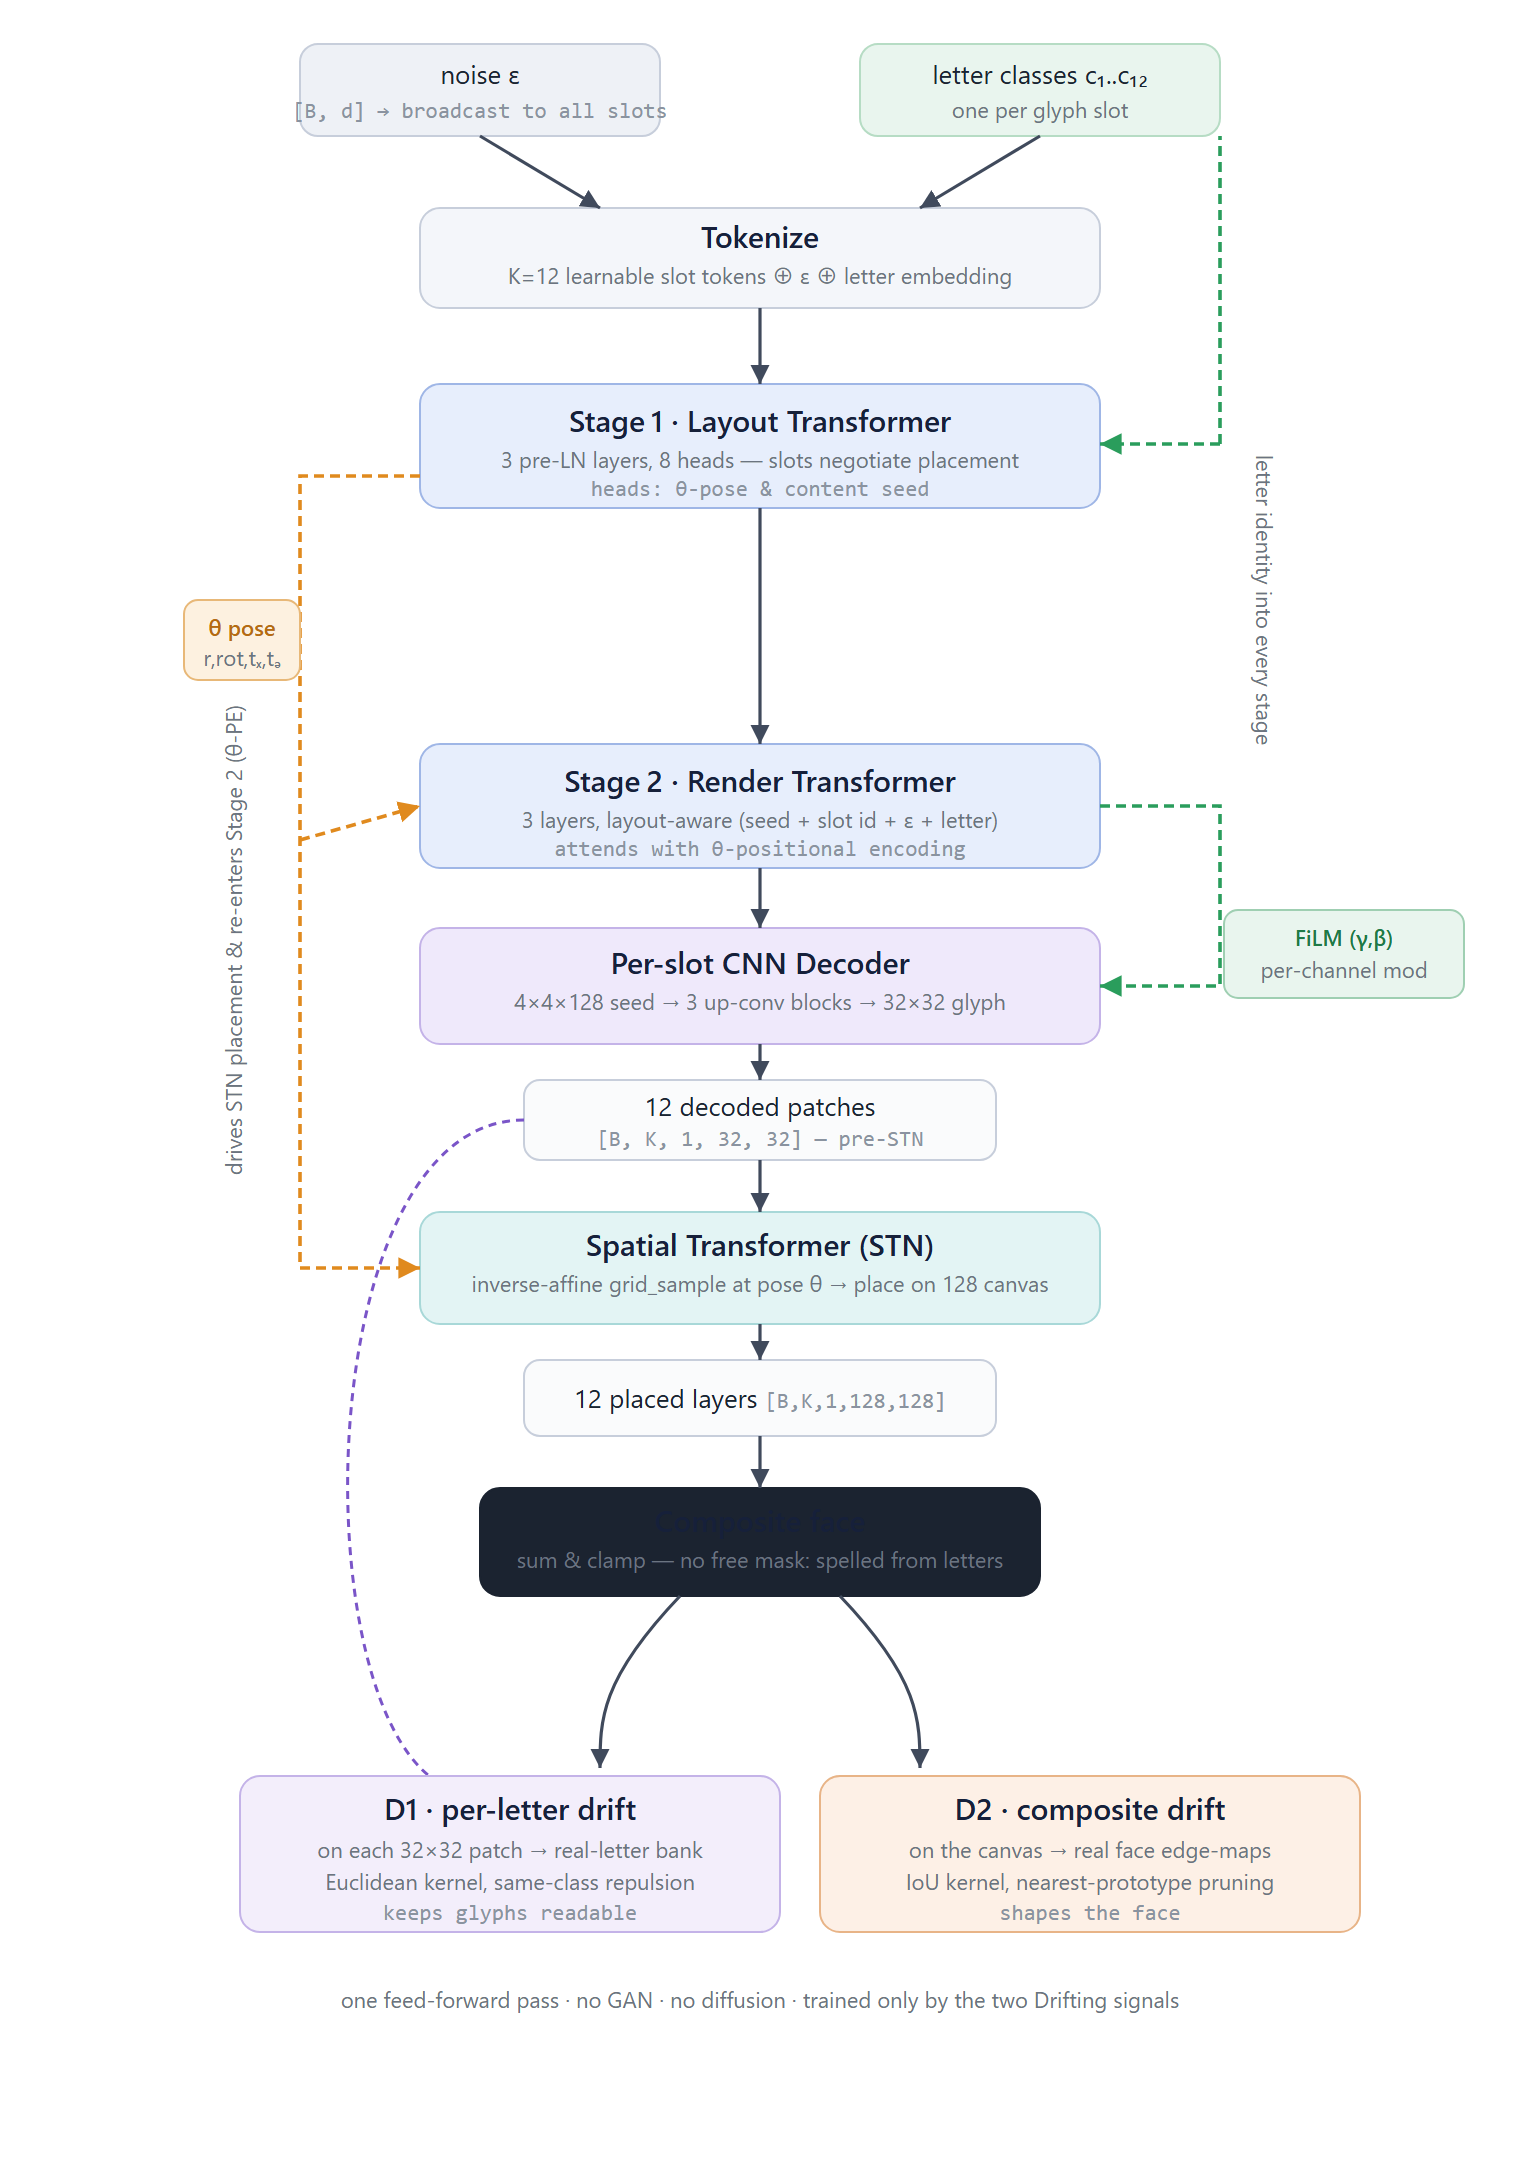
\includegraphics[height=0.86\textheight]{figs/architecture.png}
  \caption{The generator. Noise, $K$ per-glyph slot tokens, and the $K$ letter classes feed a
  two-stage transformer; Stage~1 emits affine poses and content seeds, Stage~2 renders the glyph
  images that the STN places and sum-clamps into the canvas. The pose path (orange) entangles the
  transformer with the STN. Letter conditioning (green) enters through the embedding and the FiLM
  modulation. The two drift signals use different distances: Euclidean for glyphs, and Euclidean or
  intersection-over-union for faces.}
  \label{fig:arch}
\end{figure}

\subsection{Losses}
\label{sec:loss}
The objective is a weighted sum of a face term, a letter term, and structural regularizers. We give
the exact form of every term; $\ell_{k}$ denotes the placed ink of layer $k$ at a pixel, $I$ the
canvas, $\overline{\mathrm{ink}}_\real$ the mean ink of the real collection, and $\mathbb{E}$ a mean
over the indicated axes. Default weights are in Table~\ref{tab:hparams}.

\paragraph{Distances.}
\label{sec:kernels}
The distance $d$ inside Drifting (Alg.~\ref{alg:drift}, step 2) is modular. The two we use most are the
Euclidean distance and a soft intersection-over-union (IoU) distance,
\begin{align}
   d_{\mathrm{L2}}(x,y)&=\sqrt{\max\!\big(\|x\|^2+\|y\|^2-2\langle x,y\rangle,\,10^{-8}\big)},\\
   d_{\mathrm{IoU}}(x,y)&=1-\frac{\langle x,y\rangle}{\|x\|_1+\|y\|_1-\langle x,y\rangle+10^{-6}},
\end{align}
the latter treating pixel values as soft occupancy (intersection $=\langle x,y\rangle$, union
$=\|x\|_1{+}\|y\|_1{-}$intersection). We also implemented a Dice distance
($1{-}2\langle x,y\rangle/(\|x\|_1{+}\|y\|_1)$), a multi-scale IoU (mean of the IoU distance over the
maps average-pooled by $1,2,4\times$), a gradient-domain IoU (IoU on Sobel edge magnitudes), and a
low-frequency Euclidean distance (Fourier coefficients weighted by $1/(1{+}10|f|)$). The IoU distance
is excellent for faces but, applied to letters, collapses glyphs into region-filling strokes; we
therefore use \emph{different distances at the two levels} --- Euclidean for the glyph signal (which
preserves glyph shape) and Euclidean or IoU for the face signal. Our recommended model pairs an
\emph{IoU} face distance with a \emph{Euclidean} glyph distance: IoU gives the best and most stable
faces, and a strong legibility term plus a broad glyph temperature keep the placed glyphs readable
enough (Sec.~\ref{sec:results}); the all-Euclidean variant keeps letters crisper but yields looser,
noisier faces.

\paragraph{Face drift (composite level).} We flatten the canvas to a $16384$-dimensional vector, group
$C_g$ canvases together as one drift problem, and apply Alg.~\ref{alg:drift} with $C_p$ positive and
$C_n$ negative references drawn at random from the real face line-drawings (the detached siblings
within the group supply the intra-batch repulsion):
\begin{equation}
   \mathcal{L}_{\mathrm{face}} = \mathbb{E}\big[\mathcal{L}_{\mathrm{drift}}(\mathrm{vec}(I))\big],
   \qquad \text{bandwidths } R\in\{0.005,0.02,0.1\},\ \text{distance } d_{\mathrm{face}}.
\end{equation}

\paragraph{Glyph drift (per-letter level, categorical repulsion).} For each letter class $c$ we gather
all generated glyph images assigned to $c$ in the batch; each is its own drift problem. Its positive
references are $C_p^{\!\ell}$ random \emph{real} augmented letters of the \emph{same} class $c$; its
negatives are $C_n^{\!\ell}$ \emph{other generated glyphs of the same class} (self excluded,
detached). Thus a generated ``A'' is repelled only by other generated ``A''s and never by a ``B'' ---
the repulsion is categorical, preventing mode collapse \emph{within} a class without forcing different
letters apart:
\begin{equation}
   \mathcal{L}_{\mathrm{glyph}} = \frac{1}{N}\sum_{c}\sum_{i\in c}\Big\| P_i-\sg\!\big(P_i+V_p^{(c)}(P_i)-V_q^{(c)}(P_i)\big)\Big\|^2,
\end{equation}
with $V_p^{(c)}$ from real class-$c$ letters and $V_q^{(c)}$ from sibling generated class-$c$ glyphs,
Euclidean distance, the same bandwidths, normalized by the total glyph count $N$.

\paragraph{Legibility auxiliary (cross-entropy).} Because Drifting matches a \emph{distribution} and
tolerates deformation, a glyph can drift far from a canonical letter shape. We add a small
cross-entropy term from a \emph{frozen} letter classifier $f$ (Sec.~\ref{sec:auxmodels}),
$\mathcal{L}_{\mathrm{CE}}=\mathrm{CE}\big(f(P_k),c_k\big)$, that pushes each glyph to be
\emph{classified} as its target letter. The classifier is trained on the \emph{same}
aggressively-augmented letters as the glyph drift, so it rewards deformation-tolerant legibility rather
than upright, canonical glyphs. It is an auxiliary only: Drifting remains the main letter signal,
because a bare classifier loss can be satisfied by adversarial textures.

\paragraph{Structural regularizers (exact forms).}
\begin{align}
\text{region IoU:}\;
&\mathcal{L}_{\mathrm{rIoU}} = \lambda_{\mathrm{rIoU}}\,\mathbb{E}_B\!\Big[1-\tfrac{\sum_r c_r t_r}{\sum_r c_r+\sum_r t_r-\sum_r c_r t_r+10^{-6}}\Big]\\
\text{overlap:}\;
&\mathcal{L}_{\mathrm{ov}} = \lambda_{\mathrm{ov}}\,\mathbb{E}_{B,\mathrm{px}}\!\Big[\tfrac{(\sum_k\ell_k)^2-\sum_k\ell_k^2}{2}\Big]=\lambda_{\mathrm{ov}}\,\mathbb{E}\big[\textstyle\sum_{i<j}\ell_i\ell_j\big]\\
\text{coverage:}\;
&\mathcal{L}_{\mathrm{cov}} = \lambda_{\mathrm{cov}}\,\big(\bar I-\overline{\mathrm{ink}}_\real\big)^2\\
\text{sharpness:}\;
&\mathcal{L}_{\mathrm{sh}} = w_{\mathrm{sh}}\,\mathbb{E}_{\mathrm{px}}\!\big[1-4(I-\tfrac12)^2\big]\\
\text{total variation:}\;
&\mathcal{L}_{\mathrm{TV}} = \lambda_{\mathrm{TV}}\big(\mathbb{E}|I_{x,y+1}-I_{x,y}|+\mathbb{E}|I_{x+1,y}-I_{x,y}|\big)\\
\text{locality:}\;
&\mathcal{L}_{\mathrm{loc}} = \lambda_{\mathrm{loc}}\,\mathbb{E}_{B,k}\!\Big[\tfrac{\sum_p\ell_{k,p}\big((y_p-c^y_k)^2+(x_p-c^x_k)^2\big)}{\sum_p\ell_{k,p}}\Big]\\
\text{dead-layer hinge:}\;
&\mathcal{L}_{\mathrm{min}} = w_{\mathrm{min}}\textstyle\sum_{k=1}^{K}\mathrm{ReLU}\big(\tau_{\min}-\bar\ell_k\big),\quad \bar\ell_k=\mathbb{E}_{B,\mathrm{px}}[\ell_k]
\end{align}
The region term is a soft (1$-$IoU) of the canvas and a random real face after both are coarsened into
an $n{\times}n$ grid of mean-ink cells ($\mathrm{pool}_n$ averages over $128/n$-pixel blocks); it pushes
ink toward face-anatomical regions \emph{without} encoding any specific landmark. Overlap discourages
two glyphs from stacking on the same pixels (using
$\sum_{i<j}\ell_i\ell_j=\tfrac12[(\sum\ell)^2-\sum\ell^2]$); coverage matches the global ink ratio;
sharpness pushes pixels toward $\{0,1\}$; total variation removes spurious thin strokes; locality keeps
each glyph's ink spatially compact (its second central moment about its own centroid); the dead-layer
hinge penalizes any layer whose mean ink falls below a floor, preventing slots from going blank.

\paragraph{Total objective.}
\begin{equation}
\label{eq:total}
   \mathcal{L} = \underbrace{\mathcal{L}_{\mathrm{face}}+\mathcal{L}_{\mathrm{rIoU}}}_{\text{face}}
   + \underbrace{w_{\ell}\,\mathcal{L}_{\mathrm{glyph}}+w_{c}\,\mathcal{L}_{\mathrm{CE}}}_{\text{letter}}
   + \mathcal{L}_{\mathrm{ov}}+\mathcal{L}_{\mathrm{cov}}+\mathcal{L}_{\mathrm{sh}}+\mathcal{L}_{\mathrm{TV}}+\mathcal{L}_{\mathrm{loc}}+\mathcal{L}_{\mathrm{min}}.
\end{equation}
In the stable regime the face drift ($\approx5\text{--}7$) dominates, the region term is
$\approx1.35$, the glyph drift $\approx0.9$, and the cross-entropy term (large at the start,
$\approx3$) is satisfied within about $100$ steps and decays toward $0$. The face pressure is thus
roughly $5\times$ the letter pressure, which directly explains why a strong face signal bends glyphs
into strokes.

\paragraph{Adaptive letter weighting.} To control this balance precisely we optionally make
$w_\ell,w_c$ adaptive. At each step we divide each letter term by its own current value and rescale it
to a fixed target fraction of the current face pressure $F=\mathcal{L}_{\mathrm{face}}+\mathcal{L}_{\mathrm{rIoU}}$,
\begin{equation}
   w_\ell = \mathrm{clip}\Big(\rho_{\mathrm{glyph}}\,\tfrac{F}{\mathcal{L}_{\mathrm{glyph}}}\Big),\qquad
   w_c = \mathrm{clip}\Big(\rho_{\mathrm{CE}}\,\tfrac{F}{\mathcal{L}_{\mathrm{CE}}}\Big),
\end{equation}
using current stop-gradient values (no moving average), so the glyph contribution is pinned to
$\rho_{\mathrm{glyph}}F$ and the cross-entropy to $\rho_{\mathrm{CE}}F$ regardless of how the raw
magnitudes drift over training. The two letter terms are balanced \emph{independently}. We found,
however, that this adaptive scheme \emph{hurts}: it raises the letter weight precisely when the letters
are already well-formed (small loss), over-constraining them and starving the face signal. Our final
model therefore uses \emph{fixed} weights (the glyph drift at its natural scale, giving a
glyph-to-face ratio near $0.14$, and a small fixed cross-entropy weight); fixed weights have the
correct behavior automatically, since a small letter loss simply yields a small contribution
(Sec.~\ref{sec:results}).

\subsection{Data and augmentation}
\label{sec:data}
Both collections are unpaired. The exact pipelines follow; samples are shown in Fig.~\ref{fig:data}.

\paragraph{Face line-drawings (the face target).} From $20{,}000$ aligned CelebA \citep{liu2015celeba}
portraits we build binary line-drawings: (1) resize to $128{\times}128$ with area interpolation; (2)
Gaussian blur, standard deviation $1.4$ pixels; (3) Canny edge detection \citep{canny1986} with
hysteresis thresholds $(75,170)$; (4) sparsify by removing connected components smaller than $8$
pixels; (5) dilate once with a $3{\times}3$ elliptical kernel to thicken strokes into a clean
marker-pen look. The result is binary, with a mean ink fraction of about $0.275$.

\paragraph{Letter collection (the glyph target).} From EMNIST \citep{cohen2017emnist} handwritten
letters ($26$ classes) we build $2000$ pre-augmented variants per class at $32{\times}32$, in order:
(1) a \emph{coarse} elastic deformation \citep{simard2003elastic} followed by a \emph{fine} one, each a
Gaussian-smoothed random displacement field renormalized to a target root-mean-square pixel amplitude
and applied by warping
(coarse field: smoothing $\approx7.7$\,px and amplitude $\approx2.1$\,px over $10$ accumulation steps;
fine field: smoothing $\approx2.9$\,px and amplitude $\approx0.7$\,px over $8$ steps); (2) a
center-aligned affine warp with rotation up to $\pm35^\circ$, shear up to $\pm0.25$, and independent
horizontal/vertical scaling up to $\pm18\%$ (renormalized so the longer axis is unchanged, i.e.\ no
upscaling) --- translation is \emph{not} part of the affine; (3) a fit-to-canvas step that crops to the
ink bounding box, rescales the longer side to a random $55\text{--}95\%$ of the canvas, and recenters
with a small positional jitter. With probability $0.08$ a sample is drawn from an even more extreme
setting (rotations to $\pm55^\circ$, larger fields). A ``mild'' setting (used only for one ablation
classifier) roughly halves every range. This heavy yet shape-preserving augmentation teaches the
decoder a deformation-tolerant prior over each letter, which is what lets the placed glyphs bend toward
facial contours while remaining recognizable; the same augmented collection trains the legibility
classifier.

\begin{figure}[t]
  \centering
  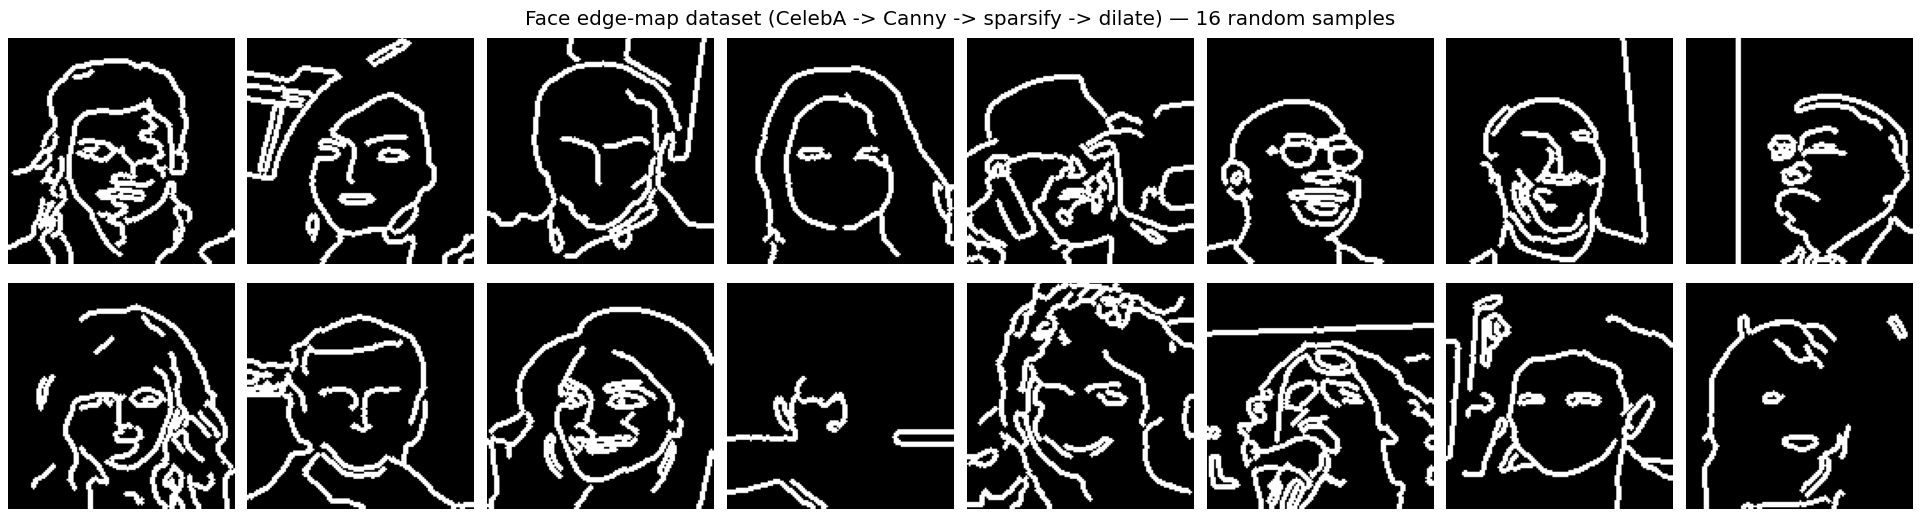
\includegraphics[width=0.96\linewidth]{figs/face_dataset_16.png}\\[4pt]
  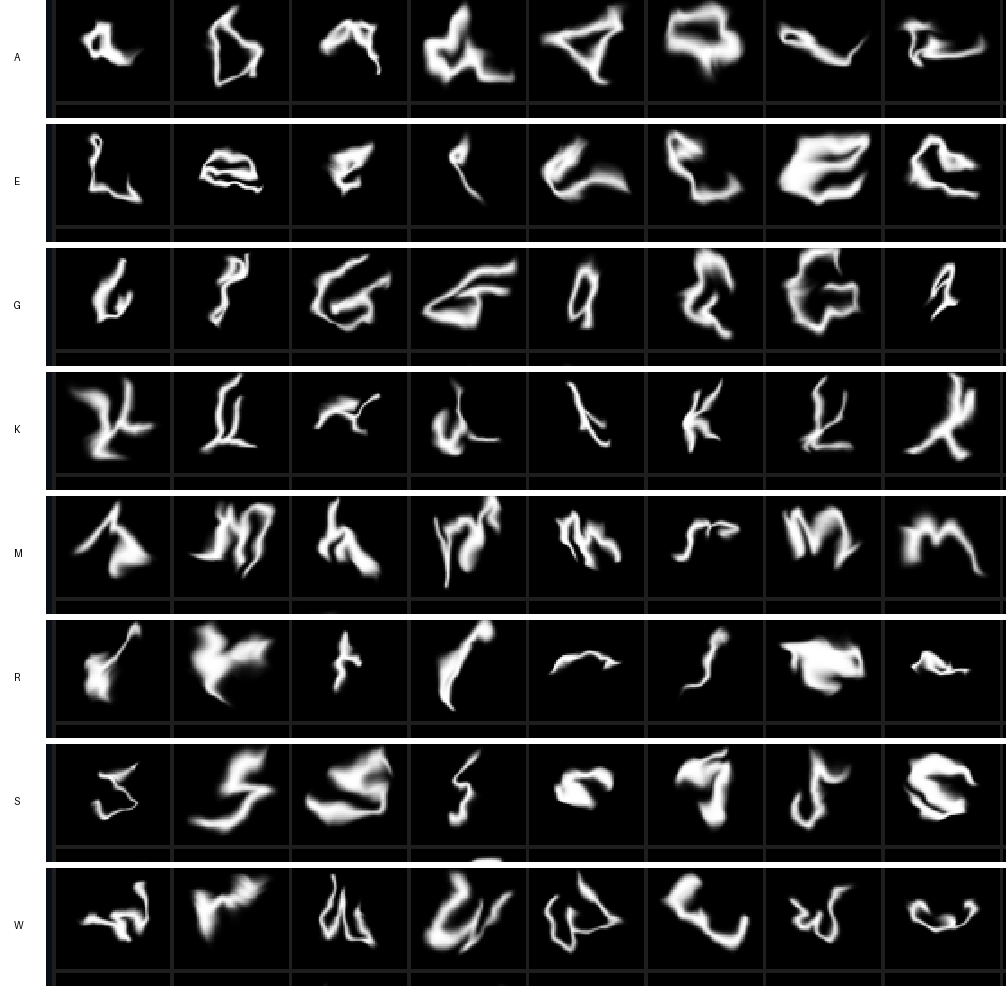
\includegraphics[width=0.78\linewidth]{figs/letter_aug_montage.png}
  \caption{\textbf{Top:} 16 random face line-drawings (CelebA $\to$ blur $\to$ Canny $\to$ sparsify
  $\to$ dilate), the face target. \textbf{Bottom:} augmented letters --- 8 variants each for 8 letters
  (EMNIST $\to$ two-stage elastic warp $\to$ affine $\to$ fit-to-canvas), the glyph target. The heavy,
  shape-preserving deformation lets a placed glyph bend toward a facial contour while staying
  recognizable.}
  \label{fig:data}
\end{figure}

\section{Experiments}
\label{sec:experiments}
\subsection{Experimental setup}
\label{sec:setup}
\paragraph{Metrics.} Because the data are sparse binary line-drawings, the usual Inception-based
Fr\'echet distance is a domain mismatch. We instead report a \textbf{kernel distance in an edge-domain
feature space}: we encode real and generated canvases with a frozen autoencoder trained on the face
line-drawings (Sec.~\ref{sec:auxmodels}), reduce its bottleneck to a $256$-dimensional vector by
average pooling, and compute the unbiased polynomial-kernel maximum mean discrepancy (KID,
$\times10^3$, lower is better) \citep{binkowski2018kid} with a block estimator over $10$ resamples. We
complement it with improved \textbf{precision and recall} \citep{kynkaanniemi2019pr} (realism vs.\
diversity). For letters we report a frozen-classifier \textbf{legibility probe}, but stress that it is
\emph{circular} when the same classifier appears in the loss. To get a meaningful number we therefore
evaluate legibility with a \emph{held-out} classifier --- one trained at a different augmentation
strength than the one used in the loss --- and complement it with visual inspection
(Table~\ref{tab:main}, last column).
\paragraph{Compute.} Each model trains on a single NVIDIA RTX PRO 6000 (96\,GB); an $8000$-step run
takes about $2$ hours. The full study --- the configurations in Table~\ref{tab:main} plus seed
replicates and abandoned directions --- used on the order of a few dozen such runs.

\subsection{Baseline: pure-drifting face generation}
\label{sec:baseline}
To isolate the cost of the letter constraint --- and to confirm that Drifting alone produces faces in
our line-drawing domain --- we first train an \emph{unconstrained} baseline that generates face
line-drawings directly, with \emph{no letters, slots, or STN}. This baseline is itself a deliverable of
the project, so we document it fully.

\paragraph{Architecture.} A noise vector ($128$ dimensions) is projected by a linear layer to a
$192{\times}4{\times}4$ feature map and upsampled by five nearest-neighbour convolutional blocks (each:
$2\times$ upsample, $3{\times}3$ convolution, group normalization, GELU) with channel widths
$192\to192\to192\to96\to48\to24$, reaching $128{\times}128$; a final $3{\times}3$ convolution to one
channel and a sigmoid produce the line-drawing. There is no autoencoder, decoder, or composition: the
single output map \emph{is} the face.

\paragraph{Loss and training.} The face drift only, using the IoU distance, bandwidths
$\{0.005,0.02,0.1\}$, $64$ positive and $16$ negative references per problem and $32$ generated samples
per problem, plus the same coverage, sharpness, and total-variation regularizers and the input-noise
smoothing. Optimization: AdamW (learning rate $2{\times}10^{-4}$, $\beta=(0.9,0.95)$), gradient-norm
clipping at $1.0$, an exponential moving average of the weights (decay $0.999$, used for all sampling),
batch size $256$, $24000$ steps, on a separate collection of $20{,}000$ \emph{thin} (non-dilated) Canny
line-drawings (Gaussian blur $1.0$, thresholds $(40,110)$, mean ink $0.105$). The kernel distance is
always measured against a model's own training collection.

\paragraph{Two settings, and why they differ.} We report two checkpoints of this baseline as
reference points; they are trained identically and differ in \emph{one} thing only --- whether the
drift target is pruned to a few nearest prototypes (Sec.~\ref{sec:overview}, modification 2). The effect
is instructive, because it exposes exactly what the drift force pulls a generated face toward. Recall
that the attraction field $V_p$ moves each generated sample toward an \emph{affinity-weighted average}
of the real references. \emph{Without} pruning, that average runs over the whole collection: since the
eyes, nose, and mouth sit at slightly different places across thousands of faces, averaging their
line-drawings smears every feature out, and the model converges to a clean but \emph{blurry mean face}
(Fig.~\ref{fig:baseline}a). \emph{With} pruning --- keeping only the $4$ nearest positive and $8$
nearest negative references per sample --- the target becomes the average of just the handful of real
faces most similar to the current generation. Those few are mutually consistent, so their average
\emph{retains} sharp eyes, nose, and mouth; the price is a mild doubled-contour artifact, which appears
where the nearest few faces have slightly offset edges and the average shows both
(Fig.~\ref{fig:baseline}b). In short, pruning trades a little contour crispness against a large gain in
feature sharpness by replacing a global mean target with a local, few-prototype one. The pruned setting
reaches a kernel distance of about $\mathbf{32.6}$ (precision $0.55$, recall $0.59$), far below any
letter-constrained model: it is the face-quality ceiling of the method, and the gap from it to the full
W2F model is the price of spelling the face out of legible glyphs.

\begin{figure}[t]
  \centering
  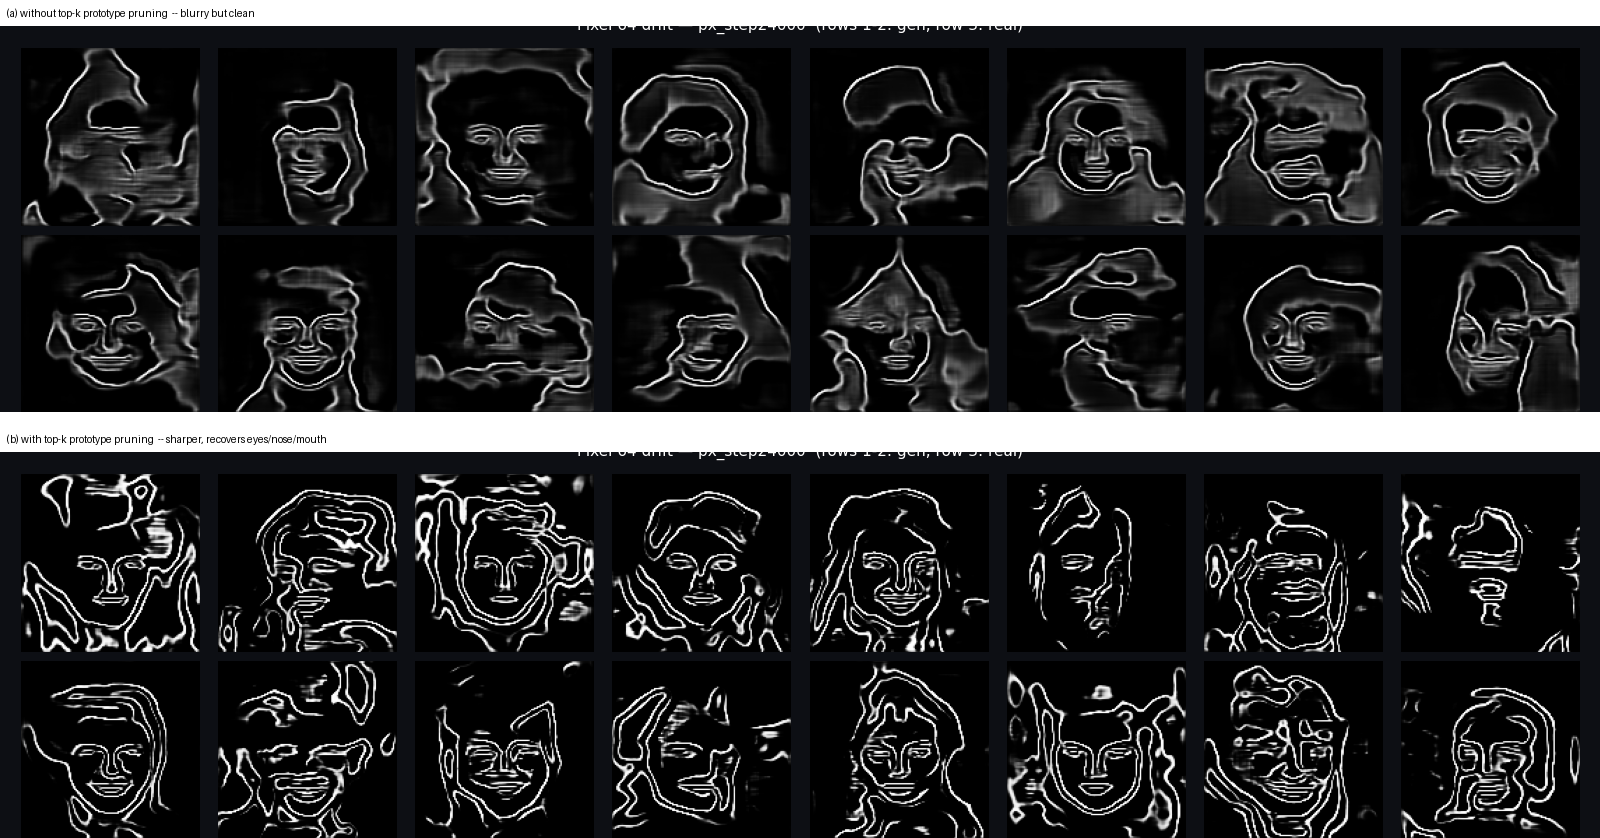
\includegraphics[width=0.98\linewidth]{figs/baseline_faces.png}
  \caption{Unconstrained pure-drifting faces (face signal only, no letters). (a) Without
  nearest-neighbour pruning: clean but blurry. (b) With pruning: sharper, with recovered eyes/nose/mouth
  (kernel distance $\approx32.6$). This is the face-quality upper bound.}
  \label{fig:baseline}
\end{figure}

\subsection{Frozen models used for evaluation}
\label{sec:auxmodels}
Two frozen models are needed to reproduce our numbers; both are trained once and then held fixed.

\paragraph{Feature extractor for the kernel distance.} A convolutional autoencoder on $128{\times}128$
line-drawings. The encoder has three stride-2 blocks (each: $4{\times}4$ convolution, group
normalization, GELU) with channel widths $1\to48\to96\to192$ (reducing $128\to16$), followed by a
$1{\times}1$ convolution to a $16{\times}16{\times}16$ bottleneck; the decoder mirrors it. It is trained
to reconstruct the line-drawings with a binary cross-entropy on the logits (positive-class weight $6$,
to counter the sparse foreground), AdamW (learning rate $2{\times}10^{-4}$), batch size $64$, about
$5000$ steps. The kernel-distance feature is this frozen bottleneck, average-pooled to $4{\times}4$ and
flattened to $256$ dimensions.

\paragraph{Letter classifier for the legibility term.} A small convolutional classifier on
$32{\times}32$ glyphs: two $3{\times}3$ convolutions ($32$ channels) and a max-pool, two more
($64$ channels) and a max-pool, then two fully-connected layers ($4096\to128\to26$), with ReLU
throughout. It is trained by cross-entropy with Adam (learning rate $10^{-3}$), batch size $256$, about
$2000$ steps, on the augmented letter collection (with a light $\pm2$-pixel shift); the heavy
deformation comes from the collection itself. We train two versions that differ \emph{only} in the
augmentation strength of their training letters, and use the one matched to the aggressively-augmented
letters: a classifier trained on mildly-augmented letters drags the generated glyphs toward upright,
canonical shapes and fights the deformation that the glyph drift is trying to produce. On its own
held-out aggressively-augmented letters the matched classifier reaches $64\%$ accuracy --- low in
absolute terms (the augmentation is severe) but adequate as a soft legibility signal.

\begin{table}[t]
  \caption{Default hyperparameters --- the recommended IoU-face configuration (kernel distance $124$).}
  \label{tab:hparams}
  \centering\small
  \setlength{\tabcolsep}{4.5pt}
  \begin{tabular}{llll}
    \toprule
    Group & Parameter & Value & Note \\
    \midrule
    Model & $K$, token width, layers, heads & 12, 320, 6 (3+3), 8 & two-stage transformer \\
          & glyph / canvas size & $32$ / $128$ & STN places glyph on canvas \\
          & $r_{\min},r_{\max}$, rotation, $d_{\max}$ & $0.10,0.40$, $\pm\pi/6$, $0.6$ & pose bounds \\
    Drift & face bandwidths / pruning & $0.005,0.02,0.1$ / $4,8$ & composite level \\
          & \textbf{face distance} & \textbf{IoU} & best/most stable faces \\
          & glyph distance / temperature & Euclidean / broad & bands $0.0125,0.05,0.25$ \\
          & gen / pos / neg (face) & 64, 64, 16 & per drift problem \\
          & pos / neg per class (glyph) & 32, 32 & same-class only \\
    Letter& glyph drift weight & 0.3 & fixed, not adaptive \\
          & \textbf{cross-entropy weight} & \textbf{0.3} & frozen aggressive classifier \\
    Struct& region IoU ($n{=}16$), overlap, coverage & 1.5, 5, 8 & placement / separation \\
          & sharpness, TV, dead-layer ($\tau,w$) & 0.5, 0.03, (.005, 150) & sharpness held constant \\
          & locality & $10^{-3}$ & per-glyph compactness \\
    Optim & lr, $\beta$, EMA, grad-clip & $2{\times}10^{-4}$, (.9,.95), .999, 1.0 & AdamW \\
          & batch, steps, sigmoid temp. & 2048, 8000, $1.0\to2.5$ & temp.\ ramps in $\rho{=}t/T$ \\
    \bottomrule
  \end{tabular}
\end{table}

\paragraph{Training details and curricula.}
\label{sec:train}
AdamW (learning rate $2{\times}10^{-4}$, $\beta=(0.9,0.95)$), gradient-norm clipping at $1.0$, an
exponential moving average of the weights (decay $0.999$, used for all evaluation), batch size $2048$,
for $8000$ steps. One quantity follows a curriculum: the output-sharpness temperature ramps linearly
$1.0\to2.5$ in normalized progress $\rho=t/T$ (applied to both the live and the averaged weights so the
averaged samples never lag); the sharpness-regularizer weight ($0.5$) and the letter weight ($0.5$) are
held constant. We checkpoint every $2000$ steps and \emph{keep every checkpoint}, because the model
peaks early (around step $6000$) and then slowly over-trains; we select the best checkpoint by the
kernel distance rather than taking the last.

\subsection{Results and benchmarking}
\label{sec:results}
\begin{table}[t]
  \caption{Benchmark. Edge-domain face kernel distance ($\times10^3$, lower better), improved
  precision/recall, and a held-out letter-legibility accuracy --- a frozen classifier trained at a
  \emph{different} augmentation strength than the one in the loss, so it is not circular (higher
  better). All at the early-peak checkpoint, $4096$ generated samples. \textbf{Top:} the pure-face
  ceiling and the FiLM\,$\times$\,face-distance ablation. \textbf{Bottom:} the letter-drift temperature
  sweep (Euclidean face $+$FiLM; the sharp row is a $5$-seed mean).}
  \label{tab:main}
  \centering\small
  \begin{tabular}{lcccc}
    \toprule
    Configuration & Kernel dist.\ $\downarrow$ & prec $\uparrow$ & rec $\uparrow$ & letter acc $\uparrow$ \\
    \midrule
    Pure-face baseline (no letters, no STN)          & $\mathbf{32.6}$ & 0.55 & 0.59 & --- \\
    \midrule
    Euclidean face, no FiLM                          & $169$ & 0.92 & 0.11 & 0.53 \\
    Euclidean face, $+$FiLM                          & $150{\pm}18$ & 0.84 & 0.20 & 0.52 \\
    IoU face, $+$FiLM~~\emph{(recommended)}          & $\mathbf{124{\pm}5}$ & 0.88 & 0.15 & 0.38 \\
    \midrule
    \multicolumn{5}{l}{\emph{Euclidean face $+$FiLM, varying letter-drift temperature:}}\\
    \quad sharp ($5$ seeds)                          & $150{\pm}18$ & 0.85 & 0.18 & 0.53 \\
    \quad medium                                     & $140$ & 0.87 & 0.18 & 0.58 \\
    \quad broad (best legibility)                    & $152$ & 0.80 & 0.22 & $\mathbf{0.66}$ \\
    \bottomrule
  \end{tabular}
\end{table}

\paragraph{The legibility--realism trade-off (main finding).} Every lever moves the model along a
single front: better faces cost legibility, and vice versa. We characterize four levers.

\paragraph{Distance.} A structural IoU face distance (with Euclidean glyphs) gives the best and most
\emph{stable} faces ($124\pm5$ over seeds, versus $150\pm18$ for the all-Euclidean model), but, caring
only about \emph{where} ink lands, bends the glyphs into face-conforming arcs (legibility $0.38$); IoU
at \emph{both} levels melts them entirely. Euclidean glyphs keep letters crisp at a higher, noisier face
distance.

\paragraph{Letter-drift temperature.} The softmax bandwidth of the glyph drift (Alg.~\ref{alg:drift}) is
a clean, previously-unexplored knob. Its effect on the \emph{letters} is robust --- a \emph{sharp}
temperature locks each glyph onto its single nearest prototype (legibility $0.53$); a \emph{broad} one
averages many into a generic, more-readable glyph ($0.66$) --- while its effect on the \emph{face}
distance is within seed noise ($150\pm18$ for the sharp setting). The reliable lever is the legibility
we trade, not the face number.

\paragraph{Legibility weight.} The best cross-entropy weight depends on the face distance. Under the
Euclidean model a small weight ($0.15$) is the sweet spot --- less noisy than $0.3$, not as weak as
$0.1$ (which is worse on faces). Under the IoU model the strong face pressure bends glyphs harder, so a
larger weight ($0.3$) is needed to keep them legible; this is the value in our recommended
configuration.

\paragraph{Pushing letters harder backfires.} Rescaling the letter contribution \emph{up} to a fixed,
larger fraction of the face pressure is strictly harmful: at glyph-to-face ratios $0.3,0.6,1.0$ the
faces collapse (kernel distances $918,703,1474$) \emph{and} the glyphs grow noisier. The operating point
near a ratio of $0.14$ is essentially the ceiling of letter pressure the faces tolerate.

\begin{figure}[p]
  \centering
  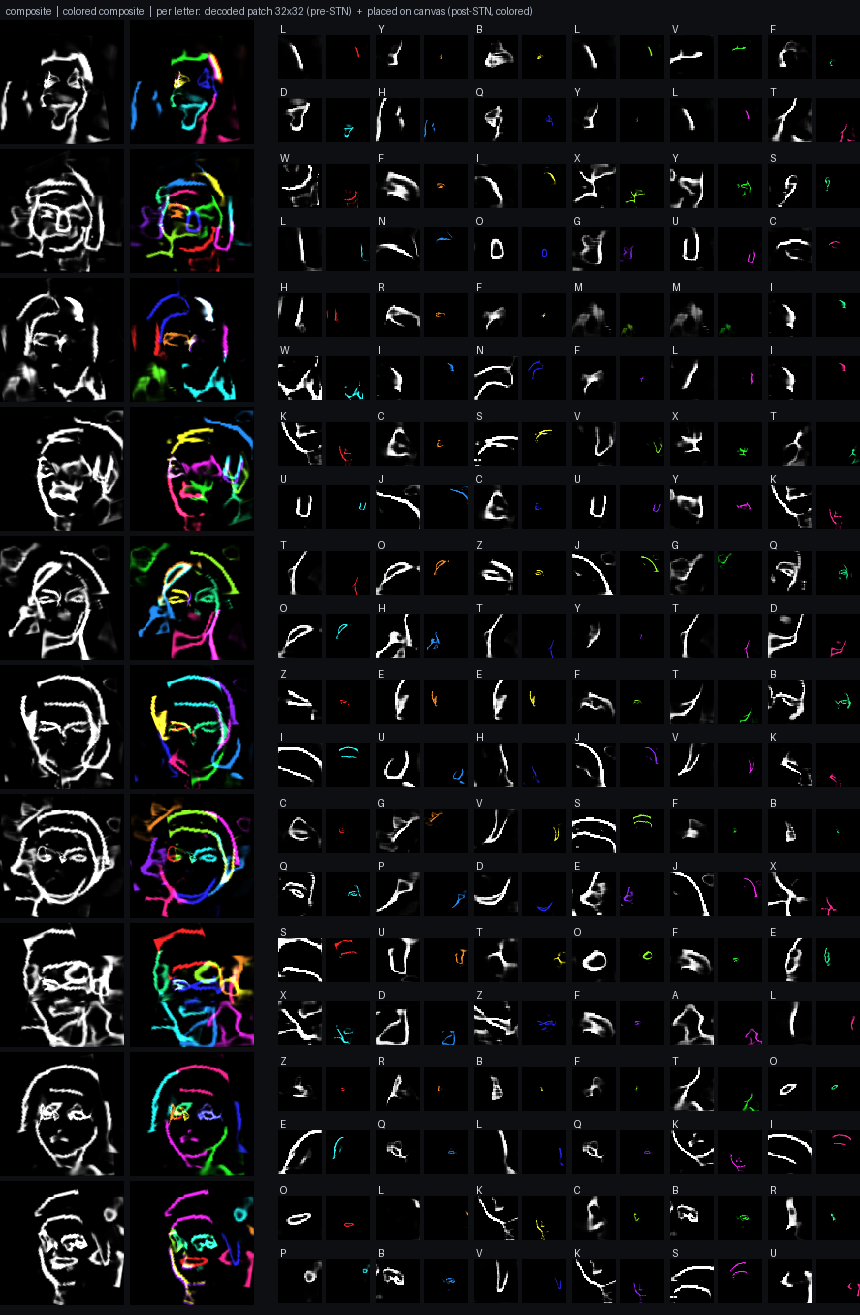
\includegraphics[width=\linewidth]{figs/gallery_fig1.png}\\[2pt]
  \caption{W2F samples (IoU face distance, broad letter temperature, legibility weight $0.3$). Each row
  is one sample: \textbf{(left)} the composite face; \textbf{(middle)} the same face colored by source
  layer; \textbf{(right)} the $K{=}12$ letters, each shown as its decoded $32{\times}32$ patch before
  the spatial transformer (left) and its colored placement on the canvas after the transformer (right).
  Part 1 of 3.}
  \label{fig:gallery1}
\end{figure}

\begin{figure}[p]
  \centering
  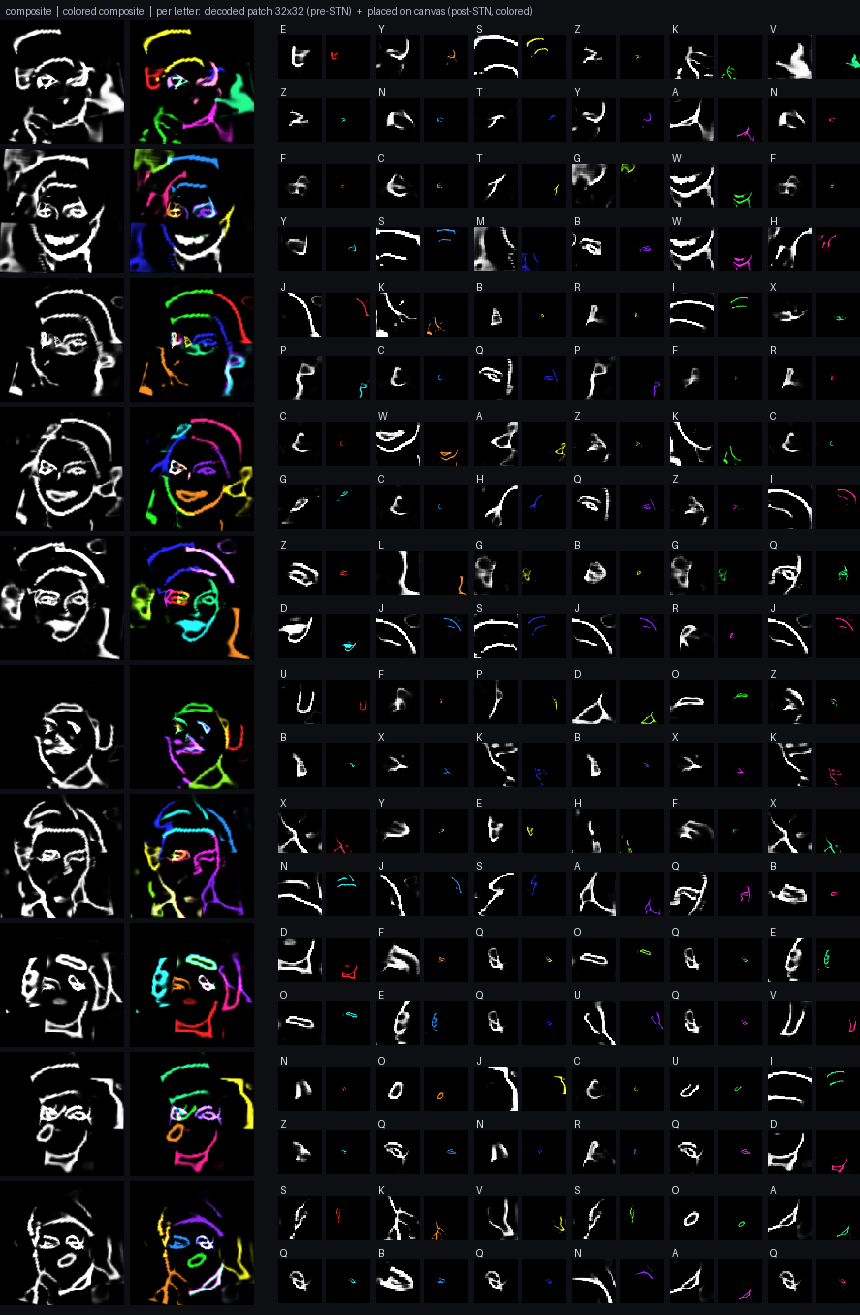
\includegraphics[width=\linewidth]{figs/gallery_fig2.png}
  \caption{W2F samples, part 2 of 3. Layout as in Fig.~\ref{fig:gallery1}.}
  \label{fig:gallery2}
\end{figure}

\begin{figure}[p]
  \centering
  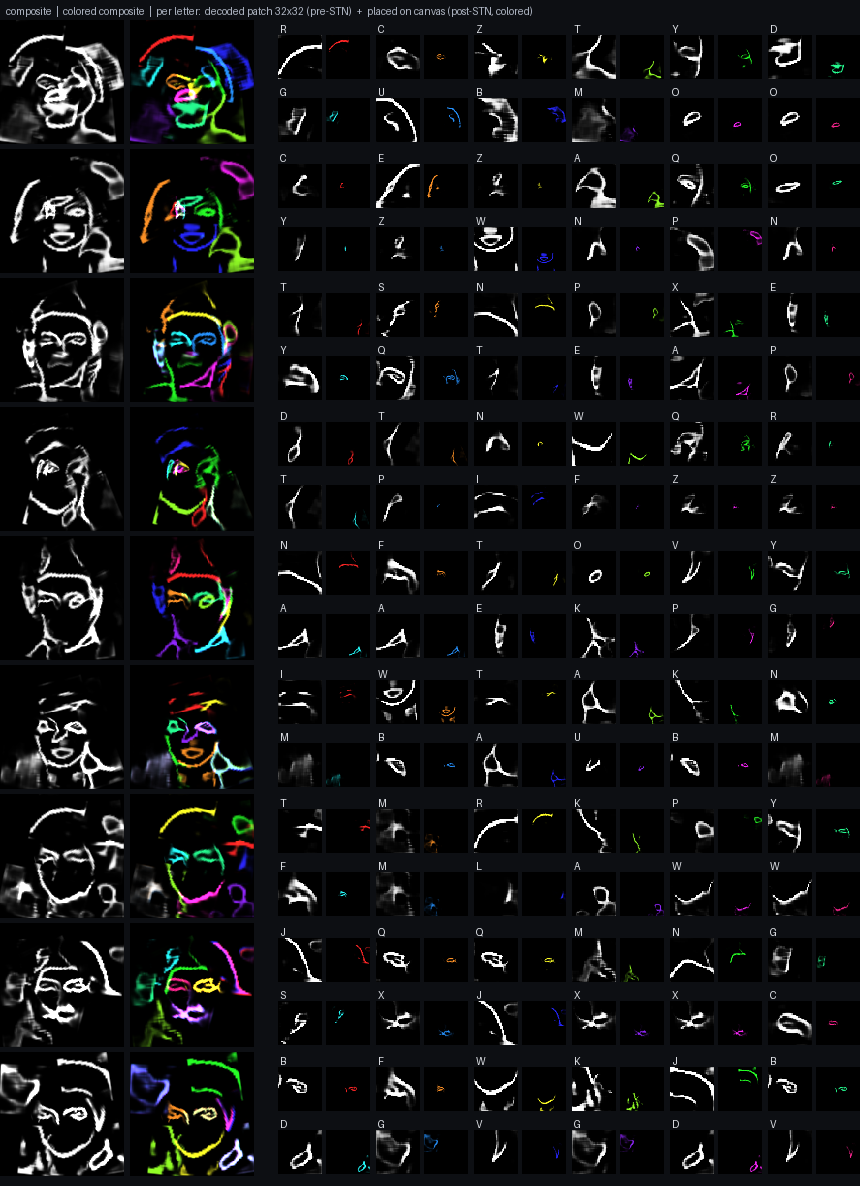
\includegraphics[width=\linewidth]{figs/gallery_fig3.png}
  \caption{W2F samples, part 3 of 3. Layout as in Fig.~\ref{fig:gallery1}.}
  \label{fig:gallery3}
\end{figure}

\subsection{Ablation: letter conditioning (FiLM)}
\label{sec:ablation}
Our main controlled ablation turns the feature-wise letter conditioning on and off with everything
else fixed (Euclidean distances, the matched legibility classifier, identical seeds and schedule).
Conditioning improves the face kernel distance by about $20$ points and roughly doubles recall ($0.22$
vs.\ $0.11$): it both sharpens structure and counters mode collapse; without it the model reaches higher
precision but markedly lower diversity (Table~\ref{tab:main}). On the letters themselves the effect is
smaller --- both variants produce the deformed, heavily-augmented style --- with conditioning giving
slightly more consistent internal structure. Figures~\ref{fig:gallery} and \ref{fig:abl_nofilm} show the
Euclidean model \emph{with} and \emph{without} feature-wise conditioning; with FiLM off the faces are
visibly less coherent.

\begin{figure}[h]
  \centering
  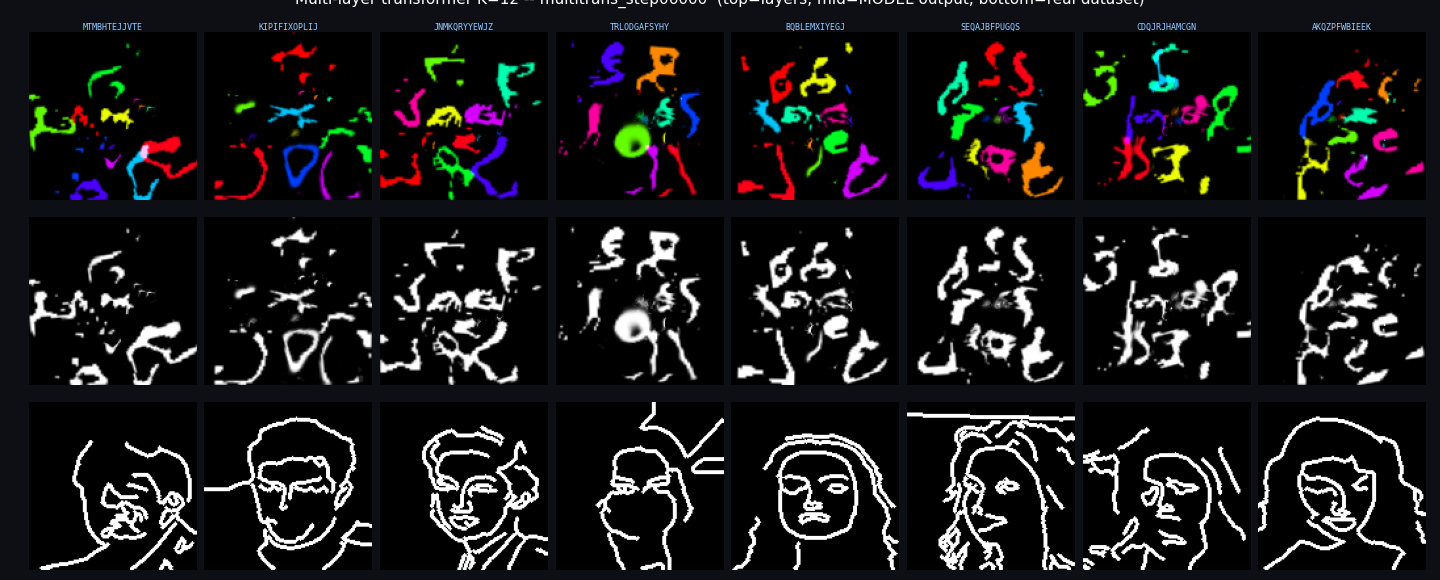
\includegraphics[width=0.98\linewidth]{figs/results_gallery.png}
  \caption{Euclidean distances \emph{with} FiLM (sharp letter temperature, legibility weight $0.15$;
  best of five seeds, kernel distance $122.6$). \textbf{Top:} the $K{=}12$ per-glyph layers (colored by
  slot). \textbf{Middle:} the composited face. \textbf{Bottom:} a real line-drawing for reference. The
  FiLM-off counterpart is Fig.~\ref{fig:abl_nofilm}.}
  \label{fig:gallery}
\end{figure}

\begin{figure}[h]
  \centering
  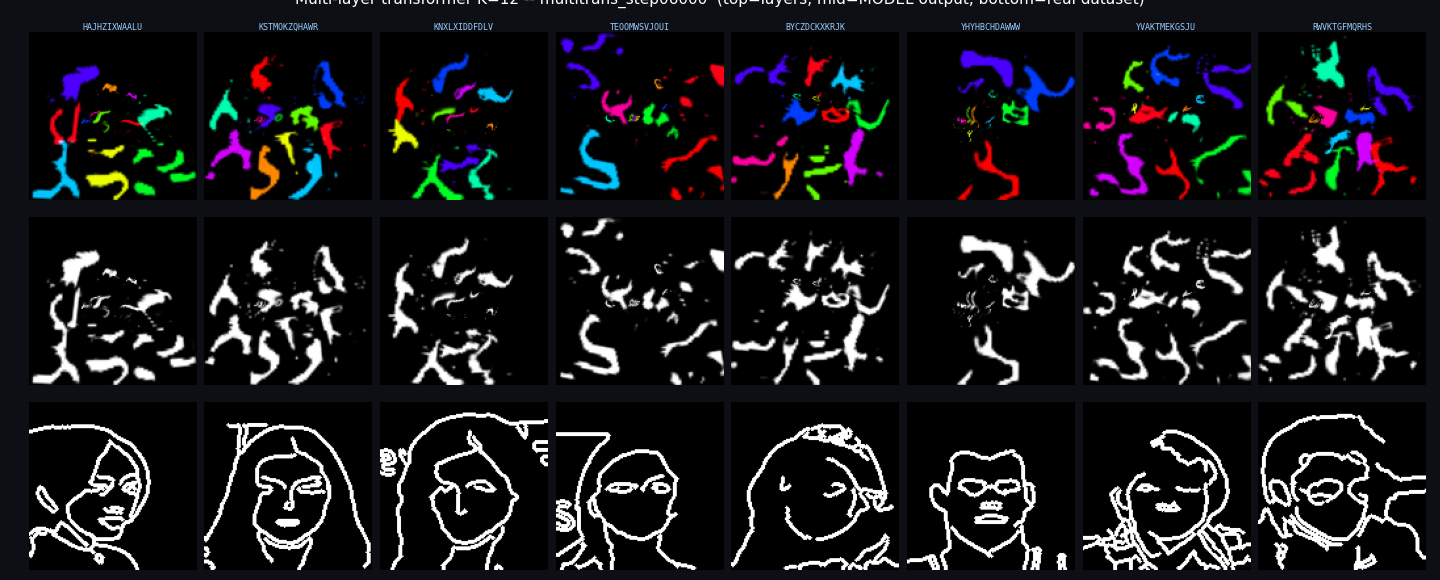
\includegraphics[width=0.98\linewidth]{figs/ablation_nofilm.png}
  \caption{Ablation --- Euclidean distances, \emph{no} feature-wise conditioning (no FiLM, no IoU).
  Same three-row layout as Fig.~\ref{fig:gallery} (colored layers / composite / real). Removing FiLM
  weakens facial structure relative to the FiLM-enabled Euclidean model.}
  \label{fig:abl_nofilm}
\end{figure}

\paragraph{Secondary observations.} (i) The legibility classifier must match the augmentation strength
of the glyph signal --- a classifier trained on mild augmentation over-canonicalizes the output. (ii)
The cross-entropy term is satisfied almost immediately and contributes little magnitude after warm-up;
once its raw value has collapsed it cannot be revived by reweighting (amplifying a near-zero loss only
injects noise), consistent with its admitting near-adversarial solutions, so we keep it a small
auxiliary. (iii) The model peaks early and over-trains, which is why we select the best checkpoint.

\section{Limitations}
\label{sec:limitations}
(i) The legibility--realism trade-off is fundamental to our setup and not fully resolved; the best
single configuration is a compromise. (ii) The letter-legibility metric is a circular proxy and
over-states readability. (iii) Results show non-trivial seed variance, so we report best-checkpoint
numbers. (iv) The number of glyphs and the canvas size are fixed; arbitrary-length strings and higher
resolutions are future work. (v) As face synthesis, the method shares general misuse considerations,
mitigated here by the abstract, glyph-built, edge-only outputs.

\section{Conclusion}
\label{sec:conclusion}
W2F shows that a one-step generator, supervised only by a particle-based Drifting objective with no
face priors and no paired data, can compose human faces out of letter glyphs. A two-stage transformer
co-adapted with a spatial transformer provides the layout, feature-wise conditioning injects letter
identity, and two-level Drifting --- with different distances for letters and faces --- plus a small
legibility term balances ``looks like a letter'' against ``looks like a face''. The remaining tension
between legibility and realism is, we argue, the core scientific content of the problem, and we
characterize the levers --- distance choice, letter weight, and classifier matching --- that move along
it.

\begin{ack}
The implementation and a draft of this paper were produced with Claude Code (Anthropic), under the
authors' direction; the authors designed the experiments, made all research decisions, and verified the
reported results.
\end{ack}

\small
\bibliographystyle{plainnat}
\bibliography{references}

\appendix
\section{Detailed experiment configurations}
\label{app:configs}
All five models share the base recipe of Sec.~\ref{sec:setup} and Table~\ref{tab:hparams} (two-stage
transformer, $K{=}12$, multi-bandwidth drift, AdamW, EMA, sum-then-clamp composition); the pure-face
baselines drop the letters, slots, and STN entirely and generate the $128{\times}128$ line-drawing
directly (Sec.~\ref{sec:baseline}). Tables~\ref{tab:app_letter} and \ref{tab:app_pure} give the full
configurations of, respectively, the three letter-constrained models and the two pure-face baselines.

Reported numbers use the early-peak checkpoint selected by the kernel distance. Rows whose value is
shared by all columns are centered across them; the rows that distinguish the configurations are in
bold.

\begin{table}[h]
  \caption{The three letter-constrained models (Sec.~\ref{sec:results}): the recommended IoU-face model
  and the two ablations.}
  \label{tab:app_letter}
  \centering\small
  \begin{tabular}{lccc}
    \toprule
     & Recommended & Ablation & Ablation \\
     & (IoU$+$FiLM) & (Euclid.\ $+$FiLM) & (Euclid., no FiLM) \\
    \midrule
    slots $K$ / token width        & \multicolumn{3}{c}{12 / 320} \\
    transformer layers / heads     & \multicolumn{3}{c}{6 (3$+$3) / 8} \\
    glyph / canvas size            & \multicolumn{3}{c}{$32$ / $128$} \\
    pose bounds $r,\mathrm{rot},d_{\max}$ & \multicolumn{3}{c}{$[0.10,0.40],\ \pm\pi/6,\ 0.6$} \\
    \midrule
    \textbf{face distance}         & IoU & Euclidean & Euclidean \\
    \textbf{face top-$k$ (pos,neg)}& $4,8$ & --- & --- \\
    glyph distance                 & \multicolumn{3}{c}{Euclidean} \\
    \textbf{glyph temperature}     & $.0125,.05,.25$ & $.0025,.01,.05$ & $.005,.02,.1$ \\
    face bandwidths                & \multicolumn{3}{c}{$0.005,0.02,0.1$} \\
    \textbf{FiLM conditioning}     & yes & yes & no \\
    \textbf{cross-entropy weight}  & 0.3 & 0.15 & 0.3 \\
    glyph drift weight (fixed)     & \multicolumn{3}{c}{0.3} \\
    gen / pos / neg (face)         & \multicolumn{3}{c}{64 / 64 / 16} \\
    pos / neg per class (glyph)    & \multicolumn{3}{c}{32 / 32} \\
    region-IoU / overlap / cov     & \multicolumn{3}{c}{1.5 / 5 / 8} \\
    sharpness / TV / locality      & \multicolumn{3}{c}{0.5 / 0.03 / $10^{-3}$} \\
    sigmoid temp.\ (curriculum)    & \multicolumn{3}{c}{$1.0\to2.5$} \\
    \midrule
    optimizer                      & \multicolumn{3}{c}{AdamW} \\
    learning rate                  & \multicolumn{3}{c}{$2\times10^{-4}$} \\
    $\beta_1,\beta_2$              & \multicolumn{3}{c}{0.9,\ 0.95} \\
    gradient clip (norm)           & \multicolumn{3}{c}{1.0} \\
    EMA decay                      & \multicolumn{3}{c}{0.999} \\
    batch (generated / step)       & \multicolumn{3}{c}{2048} \\
    steps (peak $\approx 6000$)    & \multicolumn{3}{c}{8000} \\
    \bottomrule
  \end{tabular}
\end{table}

\begin{table}[h]
  \caption{The two pure-face baselines (Sec.~\ref{sec:baseline}): a convolutional generator with no
  letters, slots, or STN, trained with the face drift only on thin (non-dilated) Canny line-drawings.}
  \label{tab:app_pure}
  \centering\small
  \begin{tabular}{lcc}
    \toprule
     & no pruning & top-$k$ pruning \\
    \midrule
    generator                      & \multicolumn{2}{c}{noise $\to$ fc $\to$ 5 nearest-upsample conv blocks} \\
    base width / noise dim         & \multicolumn{2}{c}{192 / 128} \\
    channel widths                 & \multicolumn{2}{c}{$192,192,192,96,48,24$} \\
    output                         & \multicolumn{2}{c}{$128{\times}128$ sigmoid map} \\
    \midrule
    face distance                  & \multicolumn{2}{c}{IoU} \\
    \textbf{face top-$k$ (pos,neg)}& none & $4,8$ \\
    bandwidths                     & \multicolumn{2}{c}{$0.005,0.02,0.1$} \\
    gen / pos / neg                & \multicolumn{2}{c}{32 / 64 / 16} \\
    coverage / sharpness / TV      & \multicolumn{2}{c}{5 / 1.0 / 0.03} \\
    input-noise smoothing          & \multicolumn{2}{c}{0.1} \\
    \midrule
    optimizer                      & \multicolumn{2}{c}{AdamW} \\
    learning rate                  & \multicolumn{2}{c}{$2\times10^{-4}$} \\
    $\beta_1,\beta_2$              & \multicolumn{2}{c}{0.9,\ 0.95} \\
    gradient clip (norm)           & \multicolumn{2}{c}{1.0} \\
    EMA decay                      & \multicolumn{2}{c}{0.999} \\
    batch                          & \multicolumn{2}{c}{256} \\
    steps                          & \multicolumn{2}{c}{24000} \\
    training data                  & \multicolumn{2}{c}{thin Canny edges (blur $1.0$, thresholds $40/110$)} \\
    \bottomrule
  \end{tabular}
\end{table}

\end{document}
